%%%%%%%%%%%%%%%%%%%%%%%%%%%%%%%%%%%%%%%%%%%%%%%%%%%%%%%%%%%%%%%%%%%%%%
%%                    Assignment
%%%%%%%%%%%%%%%%%%%%%%%%%%%%%%%%%%%%%%%%%%%%%%%%%%%%%%%%%%%%%%%%%%%%%%

\subsection{\glyph{Assignment}}\label{sec:assignment}

\glyph{Assignment} is used to describe the setting of a state variable to a certain value. The assignment, represented by an harpoon arrow, goes from a variable value, represented by a floating \glyph{state variable} to a variable identification, represented by a \glyph{state variable} attached to the entity affected by the assignment.  The result of an assignment is represented by \glyph{outcomes}, that is by filled dots on the arrow. The result of an \glyph{assignment} can be represented by any number of \glyph{outcomes}.

\question{NLN}{The arrowhead of assignment is currently the same than of interactions. It was suggested that we either one or the other or both. But no single combination was really esthetically nice.}

\begin{description}
 \item[SBO]\mbox{}\\ non-applicable
 \item[origin]\mbox{}\\ A state-variable (section \ref{sec:stateVariable}) on its own containing a variable value.
 \item[target]\mbox{}\\ A state-variable (section \ref{sec:stateVariable}) carried by a interactor (section \ref{sec:interactors}), containing a variable identification.
 \item[end-points]\mbox{}\\ The target extremity of an \glyph{assignment} carries an harpoon arrowhead.
 \end{description}

\begin{center}
\scalebox{0.5}{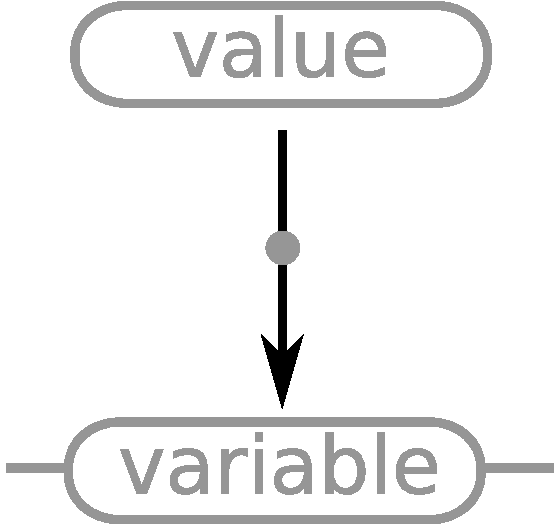
\includegraphics{images/assignment}}
\end{center}
% 
% The following example illustrates the phosphorylation of the protein phosphatase inhibitor DARPP-32 on the threonine 34.
% 
% \begin{center}
% \scalebox{0.5}{\includegraphics{images/assignment-example1.eps}}
% \end{center}
% 
% The following example illustrates two alternative assignments of the state variable ``pore'' or the nAChR. The assignment of the value ``open'' is stimulated by nicotine, while the assignement of the value ``desens'' (desensitised) is stimulated by curare. 
% 
% \begin{center}
% \scalebox{0.5}{\includegraphics{images/assignment-example2.eps}}
% \end{center}

\normalcolor

\newpage